\wysubtitle{logos.pdf}{出题：物理讲师 \textsf{Axia}}
{https://h5.qun.qq.com/s/WRps3LNC8K}{HDU 物理营}
{http://weixin.qq.com/r/mhKYgFTEMQlOrRDj90eI}{未央学社公众号}
\begin{flushleft}
    \kaishu\qquad 本资料仅作为模拟练习之用，目的是为了帮助大家更有效地复习，并减轻对考试的担忧。请正确的对待此资料，其旨在辅助复习，而非预示具体的考试内容。我们鼓励同学们认真复习，大学学习主打理解，而非刷题，期望大家在期中考试中取得优异成绩。
\end{flushleft}

\section{选择题（每题3分，共27分）}
\begin{choice}{C}[四个量子数]
    在原子的L壳层中，电子可能具有的四个量子数$(n,l,m_l,m_s)$是
\begin{tasks}[label=\roman*.](4)
    \task $(2,0,1,1/2)$
    \task $(2,1,0,-1/2)$
    \task $(2,1,1,1/2)$
    \task $(2,1,-1,-1/2)$
\end{tasks}
\begin{tasks}(4)
    \task 只有i, ii是正确的
    \task 只有ii, iii是正确的
    \task 只有ii, iii, iv是正确的
    \task 全部是正确的
\end{tasks}
\end{choice}
\solute0
\begin{solution}*
    四个量子数：$n$确定时，$l=0,1,2,\cdots,n-1;\ m_l=0,\pm 1,\cdots,\pm l;\ m_s=\pm1/2$.\sokka{C}
\end{solution}

\begin{choice}{C}[光的偏振]
分别使光强均为$I_0$的平面偏振光和自然光先后通过两个偏振片$P_1$和$P_2$. $P_1$和$P_2$的偏振化方向与原入射光光矢量振动方向的夹角分别是$\alpha$和$90^{\circ}$，则通过这两个偏振片后的光强$I$是
\begin{tasks}(2)
    \task $\frac{1}{2}I_0\cos^2{\alpha},\ \frac12I_0\cos^2\alpha$
    \task $0,\ I_0\sin^2\alpha$
    \task $\frac{1}{4}I_0\sin^2\ab(2\alpha),\ \frac12I_0\sin^2\alpha$
    \task $\frac{1}{4}I_0\sin^2{\alpha},\ I_0\cos^2\alpha$
\end{tasks}
\end{choice}
\solute0
\begin{solution}
\begin{itemize}
    \item 偏振光透过后光强$I_1=I_0\cos^2{\alpha}\cos^2{\ab(\frac{\pi}{2}-\alpha)}=I_0\cos^2\alpha\sin^2\alpha=\frac{1}{4}I_0\sin^2{\ab(2\alpha)}$.
    \item 自然光透过偏振片1后光强减半，透过偏振片2后光强$I=\frac12I_0\cos^2\ab(\frac\pi2-\alpha)=\frac12I_0\sin^2\alpha$.\sokka{C}
\end{itemize}
\end{solution}

\begin{choice}{A}[弹簧振子]
一质量为$m$的滑块，两边分别与劲度系数为$k_1$和$k_2$的轻弹簧联接，两弹簧的另外两端分别固定在墙上．滑块$m$可在光滑的水平面上滑动，$O$点为系统平衡位置．将滑块$m$向右移动到$x_0$，自静止释放，并从释放时开始计时．取水平向右为正方向，则其振动方程为？
\begin{tasks}(2)
    \task $x_0\cos\sqrt{\frac{k_1+k_2}{m}}t$
    \task $x_0\cos\sqrt{\frac{k_1k_2}{m\ab(k_1+k_2)}}t$
    \task $x_0\cos\sqrt{\frac{k_1+k_2}{m}}t+\pi$
    \task $x_0\cos\ab[\sqrt{\frac{k_1k_2}{m\ab(k_1+k_2)}}t+\pi]$
\end{tasks}
\end{choice}
\solute0
\begin{solution}
\begin{itemize}
    \item 两弹簧均连接在物块上且对物块的回复力方向相同，所以二者并联，系统角频率$\omega^2=(k_1+k_2)/m$.
    \item 初始时刻$x=x_0$，所以初相$\varphi=0$，物块的运动方程为$x=x_0\cos{\ab(\sqrt{\frac{k_1+k_2}{m}}t)}$. \sokka{A}
\end{itemize}
\end{solution}

\vskip-2ex
\begin{paracol}{2}
\begin{choice}{B}[波的能量]
    图示为一平面简谐机械波在$t$时刻的波形曲线.若此时$A$点处媒质质元的振动动能在增大，则
    \begin{tasks}(2)
        \task $A$点处质元的弹性势能在减小
        \task 波沿$x$轴负方向传播
        \task $B$点处质元的振动动能在增大
        \task 各点能量密度都不随时间变化
    \end{tasks}
\end{choice}
\switchcolumn\centering
\vfill
    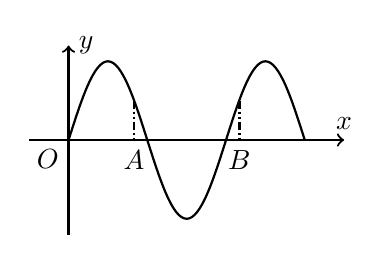
\begin{tikzpicture}
        \draw [thick,->] (-0.5,0)--(3.5,0) node [anchor=south] {$x$};
        \draw [thick,->] (0,-1.2)--(0,1.2) node [anchor=west] at (0,1.2) {$y$};
        \draw [thick] (0,0) sin (0.5,1) cos (1,0) sin (1.5,-1) cos (2,0) sin (2.5,1) cos (3,0);
        \node [anchor=north east] at (0,0) {$O$};
        \draw [thick,densely dash dot dot] (0.83,0.5)--(0.83,0) node [anchor=north] {$A$};
        \draw [thick,densely dash dot dot] (2.17,0.5)--(2.17,0) node [anchor=north] {$B$};
    \end{tikzpicture}
\vfill
\end{paracol}
\vspace{-.75em}
\begin{solution}
    \begin{itemize}
        \item $A$点的振动动能在增大，所以$A$点在靠近平衡位置，波沿$x$轴负方向传播，B项正确
        \item 波沿$x$轴负方向传播，由图可知$B$点在远离平衡位置，其振动动能在减小，C项错误
        \item 根据机械波的特性：动能和势能同时增大或减小，能量密度随时间变化，A、D项错误
    \end{itemize}
    \sokka{B}
\end{solution}

\begin{choice}{D}
    用频率分别为$\nu_1,\ \nu_2$的单色光照射某种金属时，测得的饱和光电流分别为$I_1,\ I_2$. 若$I_1>I_2$，则
\begin{tasks}(4)
    \task $\nu_1>\nu_2$
    \task $\nu_1<\nu_2$
    \task $\nu_1=\nu_2$
    \task $\nu_1,\ \nu_2$的大小无法确定
\end{tasks}
\end{choice}
\begin{solution}*
    饱和光电流大小与入射光强度有关，与入射光频率无关（出射电子最大初动能才与入射光频率有关）.
\end{solution}

\begin{choice}{A}
    设在某参考系下测得某微观粒子的总能量是它的静止能量的$\gamma$倍，则其运动速度大小为多少？若在\textbf{此}参考系下测得其寿命为$\tau_0$，则在\textbf{与其相对静止的参考系下}测得其寿命为多少？
\begin{tasks}(4)
    \task $\frac c\gamma\sqrt{\gamma^2-1},\ \frac{\tau_0}{\gamma}$
    \task $\frac c\gamma\sqrt{1-\gamma^2},\ \gamma\tau_0$
    \task $\frac{c}{\gamma-1},\ \gamma\tau_0$
    \task $\frac{c}{\gamma+1}\sqrt{\gamma(\gamma+2)},\ \frac{\tau_0}{\gamma}$
\end{tasks}
\end{choice}
\solute1
\begin{solution}*
    $E=\gamma m_0c^2=m_0c^2/\sqrt{1-v^2/c^2},\ v=c\sqrt{\gamma^2-1}/\gamma$. $\tau_0=\tau/\sqrt{1-v^2/c^2},\ \tau=\tau_0/\gamma$.
\end{solution}

\begin{choice}{A}[迈克尔逊干涉仪]
    在迈克尔逊干涉仪的一条光路中，放入一折射率为$n$，厚度为$d$的透明薄片，放入后，这条光路的光程改变了
    \begin{tasks}(5)
        \task $2\ab(n-1)d$
        \task $2nd$
        \task $2\ab(n-1)d+\frac{\lambda}{2}$
        \task $nd$
        \task $\ab(n-1)d$
    \end{tasks}
\end{choice}
\begin{solution}*
    迈克尔逊干涉仪光路上的某点光碰到反射镜后会再次经过此处，故原来的光程为$2d$；现在加入了透明薄片，使得这里的光程为$2nd$，故光程差为$2\ab(n-1)d$.\sokka{A}
\end{solution}

\vskip-2ex
\begin{paracol}{2}
    \begin{choice}{A}[双缝干涉]
        如图所示，用波长$\lambda=\qty{600}{\nm}$的单色光做杨氏双缝实验，在$P$处产生第5级明纹极大，现分别将折射率$n_1=1.75$和$n_2=1.25$的等厚薄透明玻璃片盖在两条缝上，此时$P$处变成第一级明纹极大的位置，则玻璃片厚度为
        \begin{tasks}(4)
            \task $\qty{4.8e-4}{\cm}$
            \task $\qty{6.0e-4}{\cm}$
            \task $\qty{7.2e-4}{\cm}$
            \task $\qty{8.4e-4}{\cm}$
        \end{tasks}
    \end{choice}
    \switchcolumn\centering
    \vfill
    \begin{tikzpicture}[scale=0.83]
        \draw [thick] (0,1.5)--(0,0.55);
        \draw [thick] (0,0.45)--(0,-0.45);
        \draw [thick] (0,-0.55)--(0,-1.5);
        \draw [loosely dash dot] (-0.8,0)--(5,0);
        \draw [thick] (4.5,1.8)--(4.5,-1.8);
        \fill [H6,opacity=0.4] (0,0.9) rectangle (0.2,0.1);
        \fill [H6,opacity=0.4] (0,-0.9) rectangle (0.2,-0.1);
        \draw [thick] (0,0.5)--(4.5,1.5)--(0,-0.5);
        \node [anchor=east] at (0,0.5) {$S_1$} node [anchor=east] at (0,-0.5) {$S_2$};
        \node [anchor=west] at (4.5,1.5) {$P$};
        \node [anchor=north east] at (4.5,0) {$O$};
    \end{tikzpicture}
    \vfill
\end{paracol}
\vspace{-.75em}
\solute1
\begin{solution}
    遮住前后光程差分别为
    \[\begin{cases}
        \delta_1=5\lambda=r_2-r_1\\
        \delta_2=\lambda=[r_2+(n_2-1)e]-[r_1+(n_1-1)e]
    \end{cases}\]

    联立得$5\lambda-\lambda=\qty{2400}{\nm}=\ab(n_1-n_2)e$，得玻璃片厚度$e=\qty{4.8e-4}{\cm}$.\sokka{A}
\end{solution}

\begin{choice}{C}[弗琅禾费衍射]
    在单缝夫琅和费衍射实验中，波长为$\lambda$的单色光垂直入射在宽度为$a=6\lambda$的单缝上，对应于衍射角为$30^{\circ}$的方向，单缝处波阵面可分成的半波带数目为
    \begin{tasks}(4)
        \task 2个
        \task 4个
        \task 6个
        \task 8个
    \end{tasks}
\end{choice}
\solute1
\begin{solution}*
    由衍射公式$a\sin{\theta}=k\lambda$得$k=3$，可分成的半波带数目为$2k=6$.\sokka{C}
\end{solution}

\newpage
\section{填空题（共27分）}

\begin{paracol}{2}
\begin{problem}[平面简谐波的波函数][4]
        如图所示，一简谐波向$x$轴正向传播，波速$u=\qty{500}{\m/s},\ x_0=\qty{1}{\m}$处$P$点的振动方程为$y=0.03\cos{\ab(500\pi t-\frac{\pi}{2})}$ (SI).
    \begin{enumerate}
        \item 按图所示坐标系，写出相应的波的表达式.
        \item 在图上画出$t=0$时刻的波形曲线.
    \end{enumerate}
\end{problem}
\vspace{-.75em}
\solute0
\begin{solution}*
    $y\ab(x,t)=0.03\cos{\ab[500\pi\ab(t-\frac{x-1}{500})-\frac{1}{2}\pi]}$ (SI).
\end{solution}
\switchcolumn\centering
\vfill
\begin{tikzpicture}[scale=0.83]
    \draw [->] (-2,0)--(4,0) node [anchor=north] {$x/\unit{\m}$};
    \draw [->] (0,-1.5)--(0,2) node [anchor=west] {$y/\unit{\m}$};
    \length{(0,-0.5)}{(1.5,-0.5)}{$x_0$}{(0.5,0)}
    \draw [->] (1.5,1.5)--(2.5,1.5) node [midway,anchor=south] {$u$};
    \node [solutioncolor] at (2.5,1){\footnotesize$y\ab(x,0)=0.03\cos{\ab(\pi x-\frac{\pi}{2})}$};
    \draw [very thick,solutioncolor] (-1.5,0) sin (-0.75,-0.5) cos (0,0) sin (0.75,0.5) cos (1.5,0) sin (2.25,-0.5) cos (3,0) sin (3.75,0.5);
    \draw [solutioncolor,dashed] (0,0.5)--(0.75,0.5) node [at start,anchor=east] {$0.03$};
    \shade [ball color=2号色] (1.5,0) circle (.08) node [anchor=south] {$P$};
\end{tikzpicture}
\vfill
\end{paracol}

\vskip-2ex
\begin{paracol}{2}
    \begin{problem}[单摆][3]
        在$t=0$时刻，振幅为$A$，周期为$T$的三组单摆的状态分别如图(a)、(b)、(c)所示. 若选单摆的平衡位置为坐标原点，坐标指向正右方，则单摆做小角度摆动的振动表达式（用余弦函数表示）分别为(a)\ans{$x=A\cos\ab(\frac{2\pi}{T}t-\frac{\pi}{2})$}，(b)\ans{$x=A\cos\ab(\frac{2\pi}{T}t+\frac{\pi}{2})$}，(c)\ans{$x=A\cos{\ab(\frac{2\pi}{T}t+\pi)}$}.
    \end{problem}
    \switchcolumn\centering
    \vfill
    \begin{tikzpicture}
        \foreach \a in{0,2,4}
        \draw [thick,xshift=\a cm] (-0.8,0)--(0.8,0);
        \foreach \b in{0,2,4}
        \fill [pattern=north east lines,xshift=\b cm] (-0.75,0) rectangle (0.75,0.2);
        \draw [thick] (0,0)--(0,-3);
        \draw [->] (0.1,-3)--(0.7,-3) node [anchor=south] {$v_0$};
        \shade [ball color=H1] (0,-3) circle (0.1);
    
        \draw [thick] (2,0)--(2,-3);
        \draw [->] (1.9,-3)--(1.3,-3) node [anchor=south] {$v_0$};
        \shade [ball color=H1] (2,-3) circle (0.1);
    
        \draw [thick,dashed] (4,0)--(4,-3);
        \draw [thick] (4,0)--(2.8,-2.75) node [anchor=north] {$v_0=0$};
        \shade [ball color=H1] (2.8,-2.75) circle (0.1);
    
        \node [anchor=north] at (0,-3.2) {(a)};
        \node [anchor=north] at (2,-3.2) {(b)};
        \node [anchor=north] at (4,-3.2) {(c)};
    \end{tikzpicture}
    \vfill
\end{paracol}
\vspace{-.75em}
\begin{solution}*
    三种情况对应的相位分别为$x=0,\ v>0,\ \varphi=-\frac{\pi}{2}$；$x=0,\ v<0,\ \varphi=\frac{\pi}{2}$；$x=-A,\ v=0,\ \pi$.所以振动表达式分别为$A\cos\ab(\frac{2\pi}{T}t-\frac{\pi}{2}),\ A\cos\ab(\frac{2\pi}{T}t+\frac{\pi}{2}),\ A\cos{\ab(\frac{2\pi}{T}t+\pi)}$.
\end{solution}

\begin{problem}[光电效应][4]
    光电管的阴极用逸出功$A=\qty{2.2}{\eV}$的金属制成，今用一单色光照射此光电管，阴极发射出光电子，测得遏止电势差为$\abs{U_a}=\qty{5.0}{\eV}$. 则光电管的阴极金属的光电效应红限波长为\ans{$\qty{563.56}{\nm}$}，入射光波长为\ans{$\qty{172.20}{\nm}$}.
\end{problem}
\begin{solution}*
    红限波长$\lambda_{\max}=hc/A=\qty{563.56}{\nm}$，入射光波长$\lambda=hc/(eU_a+A)=\qty{172.20}{\nm}$.
\end{solution}

\begin{problem}[起偏角][3]
    一束自然光入射到折射率分别为$n_1$和$n_2$的两种介质的交界面上，发生反射和折射.已知反射光是完全偏振光，那么折射角$r$的值为\ans{$\pi/2-\arctan{n_2/n_1}$}.
\end{problem}
\begin{solution}*
    起偏角为$\arctan{\frac{n_2}{n_1}}$，由起偏条件$i+r=90^{\circ}$得折射角$r=\frac{\pi}{2}-\arctan{\frac{n_2}{n_1}}$.
\end{solution}

\begin{problem}[相对论能动量关系][3]
    设电子静止质量为$m_e$，将一个电子从静止加速到速率为$0.6c$，需做功\ans{$m_ec^2/4$}.
\end{problem}
\begin{solution}*
    $W=mc^2-m_0c^2=m_e/\sqrt{1-v^2/c^2}-m_ec^2=m_ec^2/4$
\end{solution}

\begin{problem}[光子][3]
    频率为$\qty{2000}{\MHz}$的一个光子的能量$E=$$\ans{\qty{8.27e-6}{\MeV}}$，动量$p=$\ans{$\qty{4.42e-33}{\kg\cdot\m^2/\s^3}$}.
\end{problem}

\begin{problem}[平面简谐波的波函数][4]
    一平面简谐波沿$Ox$轴正方向传播，波长为$\lambda$，若位于$x=-L_1$的$P_1$处质点的振动方程为$y_1=A\cos\ab(2\pi\nu t+\phi)$，则位于$x=L_2$的$P_2$处质点的振动方程为\ans{$y_2=A\cos\ab[2\pi\nu t-\frac{2\pi\ab(L_2+L_1)}{\lambda}+\phi]$}；与$P_1$处质点振动状态相同的那些点的位置为\ans{$x=-L_1+k\lambda,\ k=0,\pm 1,\pm 2,\cdots$}.
\end{problem}
\begin{solution}
    设波函数为$y=A\cos\ab[2\pi\nu\ab(t-\frac{x}{\lambda\nu})+\varphi_0]$.将$P_1$点坐标$x=-L_1$代入，得
    \[y_1=A\cos\ab[2\pi\nu\ab(t+\frac{L_1}{\lambda\nu})+\varphi_0]\]

    将上式与$P_1$点振动方程比较，得初相$\varphi_0=\phi-\frac{2\pi L_1}{\lambda}$.将$\varphi_0$代入波函数中，得该波的表达式
    \[y=A\cos\ab[2\pi\nu t-\frac{2\pi\ab(x+L_1)}{\lambda}+\phi]\]

    现在令$x=L_2$，得到$P_2$点的振动方程
    \[y_2=A\cos\ab[2\pi\nu t-\frac{2\pi\ab(L_2+L_1)}{\lambda}+\phi]\]

    与点$P_1$处质点振动状态相同的点与$P_1$点的距离应为波长的整数倍，即$x=-L_1+k\lambda,\ k=0,\pm 1,\pm 2,\cdots$.
\end{solution}

\begin{problem}[增透膜][3]
    一束波长为$\lambda=\qty{600}{\nm}$的平行单色光垂直入射到折射率为$n$的透明薄膜上，\textbf{该膜是放在空气中的}.要使\textbf{透射光}得到最大限度的\textbf{加强}，薄膜最小厚度应为\ans{$\lambda/2n$}.
\end{problem}
\begin{solution}
    \begin{itemize}
        \item \textbf{当光从光密介质射向光疏介质时，反射光没有半波损失}.所以两个表面反射光光程差为$\delta=2ne+\frac\lambda2$.
        \item 可使反射光干涉相消，即$2ne+\frac\lambda2=\frac{2k+1}{2}\lambda$. 解得$k=1$时，$e_{\min}=\frac{\lambda}{2n}$.
    \end{itemize}
\end{solution}

\section{计算题（共46分）}

\begin{problem}[平面简谐波的波函数][5]
    某质点做简谐振动，周期为$\qty{3}{\s}$，振幅为$\qty{0.5}{\m}$，$t=\qty{0.75}{\s}$时刻，质点恰好在$x=\sqrt2A/2$处并向负方向运动，求
    \begin{enumerate}
        \item 该质点的振动方程.
        \item 此振动以速度$u=\qty{5}{\m/\s}$沿$x$轴负方向传播时，形成的一维简谐波的波动方程（以平衡位置为坐标原点）.
    \end{enumerate}
\end{problem}
\begin{solution}
    \begin{enumerate}
        \item 由题意得，质点的角频率$\omega=\frac{2\pi}{T}=\frac23\pi\unit{\s^{-1}}$，质点的初相$\varphi=\frac{\pi}{4}$.故质点的振动方程为\point{1}
        \[y_0=0.5\cos\ab[\frac23\pi(t-0.75)+\frac{\pi}{4}]=0.5\cos\ab[\frac23\pi t-\frac{\pi}{4}]\eqno\point{2}\]
        \item 波动表达式$y=A\cos{\ab[\omega\ab(t+\frac{x}{u})+\varphi]}=0.5\cos{\ab[\frac23\pi\ab(t+\frac{x}{5})-\frac{\pi}{4}]}$.\point{2}
    \end{enumerate}
\end{solution}

\begin{problem}[质能方程][5]
    已知电子的静能为$\qty{0.511}{\MeV}$，若电子动能为$\qty{0.25}{\MeV}$，则它所增加的质量$\Delta m$与静止质量$m_0$的比似等于多少.
\end{problem}
\begin{solution}*
    $\frac{\Delta m}{m_0}=\frac{m-m_0}{m_0}=\frac{mc^2-m_0c^2}{m_0c^2}=\frac{\qty{0.25}{\MeV}}{\qty{0.511}{\MeV}}=48.92\%$.
\end{solution}

\begin{problem}[无限深势阱][5]
    无限深势阱中运动粒子波函数为$\psi\ab(x)=\sqrt{2/a}\sin(\pi x/a)$，求发现粒子的概率密度为最大的位置 $(0\leq x\leq a)$，并求在区间$a/4\leq x\leq3a/4$发现粒子的几率.
\end{problem}
\begin{solution}
\begin{itemize}
    \item 粒子的概率密度$\omega=\abs{\psi(x)}^2=\frac2a\sin^2\ab(\frac{\pi x}{a})$，令$\frac{\d\omega}{\d x}=0$得发现粒子的概率密度为最大位置为$x=a/2$.\point{2}
    \item $P=\int_{a/4}^{3a/4}\abs{\psi(x)}^2\d x=\frac12+\frac1\pi$.\point{3}
\end{itemize}
\end{solution}

\begin{problem}[光栅][7]
    波长$\lambda=\qty{600}{\nm}$的单色光垂直入射到一光栅上，第二级主极大衍射角为$30^{\circ}$，第三级缺级.
    \begin{enumerate}
        \item 光栅常数$d=a+b$等于多少？
        \item 透光缝可能的最小宽度$a$等于多少？
        \item 在上述$d$和$a$值下，求在衍射角$-\pi/2<\varphi<\pi/2$范围内可观察到的全部主级大的级次.
    \end{enumerate}
\end{problem}
\begin{solution}
    \begin{enumerate}
        \item 由光栅方程$(a+b)\sin30^\circ=2\lambda$得$d=2\lambda/\sin 30^\circ=\qty{2.4}{\um}$.\point{2}
        \item 由缺级条件$k=k'd/a$得$a=(a+b)/3=\qty{0.8}{\um}$.\point{2}
        \item 取衍射角两侧最大值$\varphi=\pm 90^\circ$，由光栅方程$d\sin\pm90^\circ$得$k=\pm4$. 由于$k$无法取到$4$，所以此范围内可见主极大级次为$k=0,\ \pm 1,\ \pm2$.\point{3}
    \end{enumerate}
\end{solution}

\begin{problem}[弗琅禾费衍射][8]
    波长为$\qty{760}{\nm}$的平行光垂直地入射于一宽为$\qty{0.5}{\mm}$的狭缝，若在缝的后面有一焦距为$\qty{2}{\m}$的薄透镜，使光线会聚于一屏幕上，试求
\begin{enumerate}
    \item 中央明纹和旁边第一个亮纹的宽度.
    \item 第一级明纹的位置，两侧第二级暗纹之间的距离（$\qty{1}{\nm}=\qty{e-9}{\m}$）.
    \item 若换用白光照射，其中某一光波的第四级明纹和红光（$\lambda=\qty{600}{\nm}$）的第三级明纹相重合，求这一光波的波长.
\end{enumerate}
\end{problem}
\begin{solution}
    \begin{enumerate}
        \item 中央明条纹宽度$\Delta x_0=2\lambda f/a=\qty{6.08}{\mm}.\point{1}$
        \item 第一级明纹位置$a\sin{\varphi}=\pm\ab(2k+1)\frac{\lambda}{2}$，$x_1=f_1\sin{\varphi}=\pm\qty{4.56}{\mm}$.\point{2}
        
        第二级暗纹位置$a\sin{\varphi}=\pm k\lambda$，$\Delta x_2=2\cdot\frac{2\lambda}{a}f=\qty{12.16}{\mm}$.\point{2}
        \item 明纹位置$a\sin{\varphi}=\pm\frac{2k+1}{2}\lambda$，由重合条件$\frac{2\times 3+1}{2}\lambda=\frac{2\times 4+1}{2}\lambda^{\prime}$得光波波长$\lambda^{\prime}=\frac{7}{9}\lambda=\qty{446.7}{\nm}$.\point{3}
    \end{enumerate}
\end{solution}

\begin{problem}[驻波][8]
    设入射波的表达式为$y_1=A\cos[2\pi\ab(t/T+x/\lambda)]$，在$x=0$固定端发生反射，设反射时无能量损失. 求
\begin{multicols}{2}
\begin{enumerate}
    \item 反射波的表达式.
    \item 驻波的表达式.
    \item 波腹、波节的位置.
    \item 波节两侧任意两点（距离小于$\lambda/2$）的相位差为\ans{$\pi$}.
\end{enumerate}
\end{multicols}
\end{problem}
\begin{solution}
\begin{enumerate}
    \item 到达反射端后，波的传播方向发生变化，同时因半波损失带有$\pi$的相位差.所以反射波的表达式为
    \[y_2=A\cos{\ab[2\pi\ab(\frac{t}{T}-\frac{x}{\lambda})+\pi]}\eqno\point{2}\]
    \item 驻波表达式$y=y_1+y_2=2A\cos{\ab(\frac{2\pi t}{T}+\frac{\pi}{2})}\cos{\ab(\frac{2\pi x}{\lambda}-\frac{\pi}{2})}$.\point{1}
    \item 
    波腹的位置$\cos{\ab(\frac{2\pi x}{\lambda}-\frac{\pi}{2})}=\pm 1,\ x=\frac{2k+1}{4}\lambda,\ k=0,1,2,\cdots$.\point{2}

    波节的位置$\cos{\ab(\frac{2\pi x}{\lambda}-\frac{\pi}{2})}=0,\ x=\frac{k}{2}\lambda,\ k=0,1,2,\cdots$.\point{2}
    \item 波节两侧两点处质元的振动方向相反，相位差为$\pi$.\point{1}
\end{enumerate}
\end{solution}

\begin{problem}[牛顿环][8]
    牛顿环装置透镜凸表面的曲率半径是$R=\qty{400}{\cm}$.用某单色平行光垂直入射，观察反射光形成的牛顿环，测得第5个明环的半径是$\qty{0.30}{\cm}$.
    \begin{enumerate}
        \item 求入射光的波长，当平凸透镜垂直向上缓慢平移远离平面玻璃时，可以观察到这些环状干涉条纹向中心\ans{收缩}.
        \item 若将装置浸泡在折射率$n=1.25$的溶液中，求以透镜中心为圆心在半径为$\qty{1}{\cm}$的范围内可观察到的明环数目.
        \item 第三级明纹与第七级明纹所对应的空气膜厚度之差为多少？
    \end{enumerate}
\end{problem}
\begin{solution}
\begin{enumerate}
    \item 由明环半径公式$r_k=\sqrt{\frac{\ab(2k-1)\lambda R}{2}}$得入射光的波长$\lambda=\frac{2r^2}{\ab(2k-1)R}=\qty{500}{\nm}$.\point{1+2}
    \item 相当于单色光的波长变为$\lambda'=\frac{\lambda}{n}$. 由明环半径公式，代入$r=\qty{1}{\cm}$得$k=\frac{r^2}{\lambda' R}+\frac{1}{2}=63$.\point{2}
    \item 由明环半径公式$r_k=\sqrt{\frac{2k-1}{2}\lambda R}$得第三级明纹与第七级明纹所对应的空气膜厚度之差为
    \[
    \begin{aligned}
        \Delta d&=\sqrt{R^2-r_3^2}-\sqrt{R^2-r_7^2}\xlongequal{\lambda\ll R}R\ab(1-\frac{5\lambda}{4R})-R\ab(1-\frac{13\lambda}{4R})=2\lambda=\qty{1}{\um}
    \end{aligned}\eqno\point{3}
    \]
\end{enumerate}
\end{solution}


\vskip-2.5ex
% \vfill
\rightline{/*Powered by \pkg{LiteSolution} \textsf\LaTeX~Template. Designed by WeYoung \href{https://ctan.org/home/xiamyphys}{Axia}.*/}